\documentclass{amsart}
\usepackage{amsmath,amsfonts,amssymb}
\usepackage{bm}
\usepackage{graphicx}
% Theorem environments-------------------------------------------
\newtheorem{thm}{Theorem}[section]
\newtheorem{cor}[thm]{Corollary}
\newtheorem{lem}[thm]{Lemma}
\newtheorem{prop}[thm]{Proposition}
\theoremstyle{definition}
\newtheorem{defn}[thm]{Definition}
\theoremstyle{remark}
\newtheorem{rem}[thm]{Remark}
\numberwithin{equation}{section}
% simple commands---------------------------------------------
\newcommand{\abs}[1]{\left\vert#1\right\vert}
\newcommand{\set}[1]{\left\{#1\right\}}
\newcommand{\seq}[1]{\left<#1\right>}
\newcommand{\norm}[1]{\left\Vert#1\right\Vert}
%additional-------------------------------------------------------
\newtheorem{prob}{Problem}[]
%------------------------------------------------------
\begin{document}
\title{natural evolution of behaviors in a virtual ecosystem and its validation}
\date{\today}
\author{Daeseok Lee}
\begin{abstract}
	We developed a simple 2d virtual ecosystem which have many aspects of real-world lives in their simplified form. In particular, the virtual creatures in the ecosystem have neural networks that relate their visual input to their action. Several different traits including the weight parameters of the neural networks are encoded as genotype. The evolution is not guided by some given  artificial criteria as in some other systems, but death conditions such as lack of energy or being captured by a predator naturally lead to the natural selection.   
	By measuring the performance of the gene pool at different time intervals with respect to some given tasks, we argue that our creatures were able to develop configuration of the neural networks that produce actions that better fit to their input by triggering eating and mating behaviors when they are actually needed. 
	We did it not simply by inspecting the time variation of the quantities, since the apparant trend could be just the result of changes in genotype that have nothing to do with the input-dependent operation of the neural network.
	Instead, we compared the performance measurements of the creatures with those of their input-shuffled counterparts, which we call the "mixing-input trick". A rigorous argument over the trick is presented.
   The result indicates that the normal creatures made out of the gene pool sampled after a sufficient amount of time passed in a simulation performed better than their input-shuffled counterparts statistically siginifcantly enough and to the degree approximately 10% and 7% of the average performance values respectively for the two tasks.   
   Future research projects may be suggested at least in three directions: using more complex neural network models, using more elaborate virtual ecosystem and checking for the many predictions of the existing theories of evolution. 

   
	
\end{abstract}
\maketitle
%------------------------------------------------------

\section{introduction}
	We developed a 2d virtual ecosystem that have virtual creatures with many aspects of the real-world lives such as movement, predation, food intake, metabolism, excretion, mating, genetics and nervous system. The nervous system is implemented by a kind of neural network, and it determines from the visual input which direction to head, how far to move and what to do among trying to eat, trying to predate",  trying to mate and moving, all of which require certain amount of "energy". Several traits such as weights of the neural network, maximum size, nutrient accumulation rate and maximum age are encoded in the gene, and the rule  of genetics includes random mixing and mutation. The creatures either die from being in lack of energy, being eaten by a predator or being too old. For more specific details of the ecosystem and the neural network, see Appendix A and B.
	
	In the system we developed, creatures are under strong selective pressure, as measured in Appendix C. From the selective force combined with the rule of genetics, especially mutation, we may expect a form of evolution which eventually result in traits that better fit to the environment. In particular, since the weights of the neural network are also genenotype, we may expect evolution of behaviors in a sense. 
	
	In this work, we validated this claim by devicing tasks that are designed to assess a gene pool's collective ability to eat well and mate well, and applying them to gene pools sampled at different time periods. We exploited our ability as almighty of the virtual world to control alternative explanations for the performance at those tasks, by turning on and off some features of the world such as eating, childbirth or growth.
	
	More importantly, since our aim was to assess the increased ability of the neural network to perform those tasks rather than enhanced 'default' helpful characteristics such as increased speed or increased frequency of certain behaviors, we had to find a way to simulate those default behaviors to be used as baseline. This is not obvious especially in a system like this, since 'default speed', for example, is not directly extractible from the neural network itself due to it's distributed nature and dependency on inputs. 
	
	For this purpose, we deviced a simple  general trick that we call the "mixing-input trick", which assign each creature an input that is likely in the current environment but not the one that should be given to it. By doing so, we can obstruct them from acting upon the appropriate input, while still maintaining default behavioral distribution approximately. 
	
	In the second section, our work will be compared with related works. In the third section, the experiment procedures, especially the tasks are elaborated. In the fourth section, the mixing-input trick is described and argued about in more detail. In the fifth section, the result of the experiments are interpreted. In the sixth section, validity of our method, an episode during the implementation and directions of future development are discussed. The appendices include details that might not be the interest of many readers. 

\section{Related Works}
	As we will argue, our creatures learn behavioral strategies through an evolutionary mechanism. Because of this fact, one might frame it as Genetic algorithm(GA), an optimization strategy that has been applied in a variety of subfields of computer science and engineering.(See \cite{ga_survey}, for a survey of the method. See \cite{lee} for the use for multi-agent intelligent behaviors). However, ours is quite different from it in several aspects. First of all, our system is not intended to be an AI system. As a result, the "objective" or "fitness function" for the optimization is not given purposefully, but rather naturally given by the death conditions such as lack of energy and being eaten by a predator. Also, the 'mating' is something that the creatures choose to do as a part of their intelligence, rather than enforced by the algorithm itself. 
	
	Learning behaviors in virtual ecosystem context is dealt with in \cite{sims} and \cite{jeremy}, and they could achieve sophisticated morphology and behaviors. However from our viewpoint, they are still GAs; some hand-crafted objectives are used.  

	
	
\section{experiment procedures}

The experiments are composed of two stages. In the first stage, the simulation program runs in the normal mode for a given amount of time several times. During each simulation, sample dnas of a given size are extracted with a fixed time interval. At the end, we obtain a set of gene pools for each time interval, the size of which dereases as time passes.(Because sometimes simulation terminates with creatures extinct before reaching a certain time) 

In the second stage, performance with respect to some "tasks" are measured for each dna pool in each time interval. As mentioned before, the tasks are designed to measure some specific behavioral pattern, eating and mating. For each trial of task, a set of initial creatures is generated from the sampled dna pool, and the creatures are provided with some specific circumstance in which some features of the world are turned off compared to the normal world that they have been living in, for controlling purpose. After a given amount of time passes in that special world, either the total amount of food intake trial or total number of mating trials is measure.

The following are features that are turned off:

\begin{itemize}
\item 
eating : never grow, food never taken up, never produce offspring, never die due to lack of energy 

\item
mating : never produce offspring, never die due to lack of energy 
\end{itemize}

\section{mixing input trick}
In this section, $d_{in}$ and $d_{out}$ denote the size of input(size of the visual input for our case) and the size of output(12 for our case) respectively. Then, a state of the neural network and its operation can be represented as a function $f:\mathbb{R}^{d_{in}}\to\mathbb{R}^{d_{out}}$.  

Let's say at a given moment, there are $n$ creatures moving around the world. At the moment, the creatures have neural networks $f_1,f_2,\cdots,f_n:\mathbb{R}^{d_{in}}\to\mathbb{R}^{d_{out}}$ and attain inputs $x_1,x_2,\cdots,x_n\in\mathbb{R}^{d_{in}}$. In an usual simulation or when they are in an 'experimental group', they would move and take action according to the outputs $f_1(x_1),f_2(x_2),\cdots,f_n(x_n)$ respectively, which are behaviors obtained in respond to the right input. The mixing input trick that we suggest is, when they are in a control group, making them instead act upon $f_1(x_{\sigma(1)}),f_2(x_{\sigma(2)}),\cdots, f_n(x_{\sigma(n)})$ when $\sigma:\set{1,2,\cdots,n}\to\set{1,2,\cdots,n}$ is a random permutation. The advantage of doing so can be argued as follows. 

When designing a 'task' for a gene pool, there might be a golden input-relevant behavior that we want to capture,  which can be described as an implicit score function $F:\mathbb{R}^{d_{in}}\times\mathbb{R}^{d_{out}}\to\mathbb{R}_{\ge 0}$. For example in the case of the mating task we devised, $F(x,y)$ might have a high value when $x$ indicates that a potential partner is in a certain direction and $y$  indicates the creature will stretch its genitals toward that direction. We believe that when 
\begin{equation*}
\sum_{i=1}^{n}\mathbb{E}_{x_i\sim \mathcal{D}}F(x_i,f_i(x_i))
\end{equation*}
 is large, then they would achieve a high score for the task.($\mathcal{D}$ is the distribution of inputs) It might be the reason that we have designed the experiment as such. However, such an experiment may have an unexpected side effect. There can be a function $G:\mathbb{R}^{d_{out}}\to\mathbb{R}_{\ge 0}$ such that the performance in the task also depends on 
\begin{equation*}
\sum_{i=1}^{n}\mathbb{E}_{x_i\sim\mathcal{D}}G(f_i(x_i))
\end{equation*}  
For example, $G(y)$ might represent the speed determined by $y$. In this case, the preceding quantity might have a high correlation with the performance at the mating task. Therefore, we have two quantities, only one of which we are actually interested in and the other we want to control the effect of. In other words, we might want to see what happens when we retain the latter quantity roughly while messing up the former. The resulting delta on the performance might be explained by the difference in the former quantity. Then, the degree to which the performance declined might tell something about the original magnitude of the quantity of interest.


This is precisely what the mixing input trick is supposed to enable. When we apply it, the corresponding two quantities become
\begin{equation*}
\mathbb{E}_{x_1\sim\mathcal{D}}\cdots\mathbb{E}_{x_n\sim\mathcal{D}}\mathbb{E}_{\sigma\sim S_n} \sum_{i=1}^{n}F(x_i,f_i(x_{\sigma(i)}))
\end{equation*} 
and 
\begin{equation*}
\mathbb{E}_{x_1\sim\mathcal{D}}\cdots\mathbb{E}_{x_n\sim\mathcal{D}}\mathbb{E}_{\sigma\sim S_n} \sum_{i=1}^{n}G(f_i(x_{\sigma(i)}))
\end{equation*} 
You might see that while the first quantity is messed up, probably far below to a baseline level, the second one remains still if there's no change in $\mathcal{D}$. 

A care should be taken here. In fact, the "input distribution" $\mathcal{D}$ does depend on the neural process of the creatures. We are assuming that the difference is ignorable. That is, the capture image of the world in which the creatures act upon the inputs correctly looks more or less like that of another world in which they act upon the shuffled inputs. 


\section{result and analysis}
\begin{center}
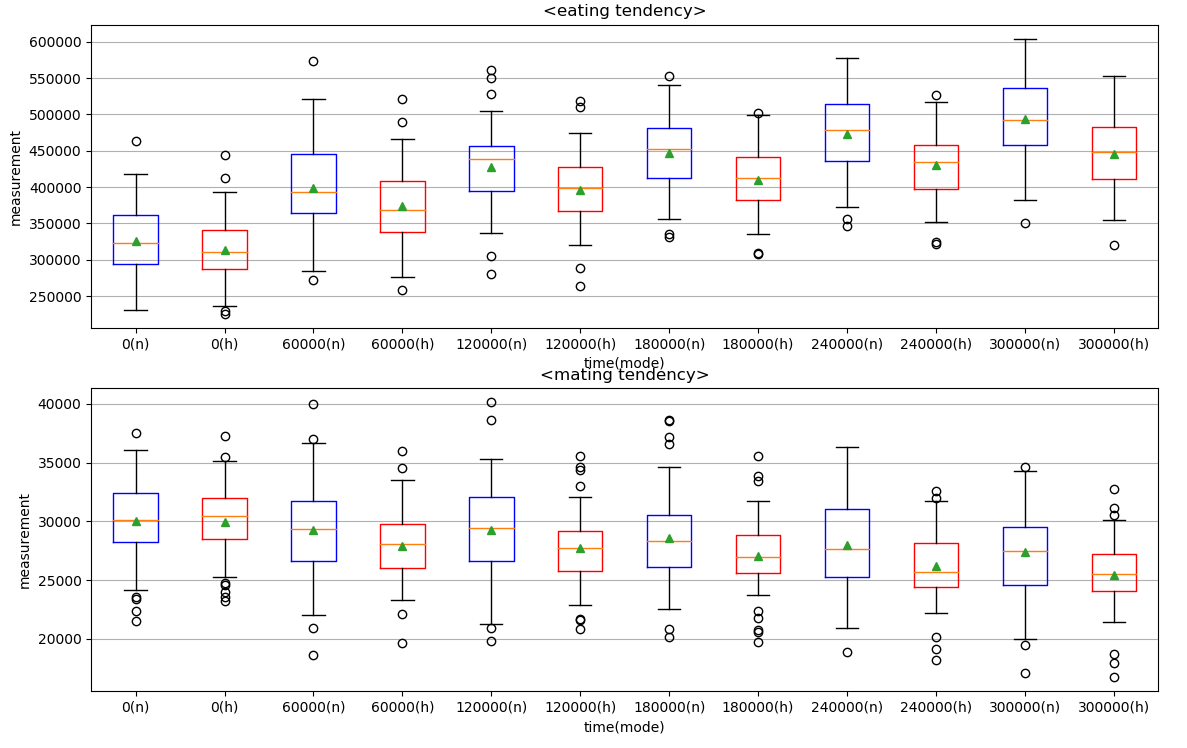
\includegraphics[scale=0.3]{images/main.png}
\end{center}
\begin{center}
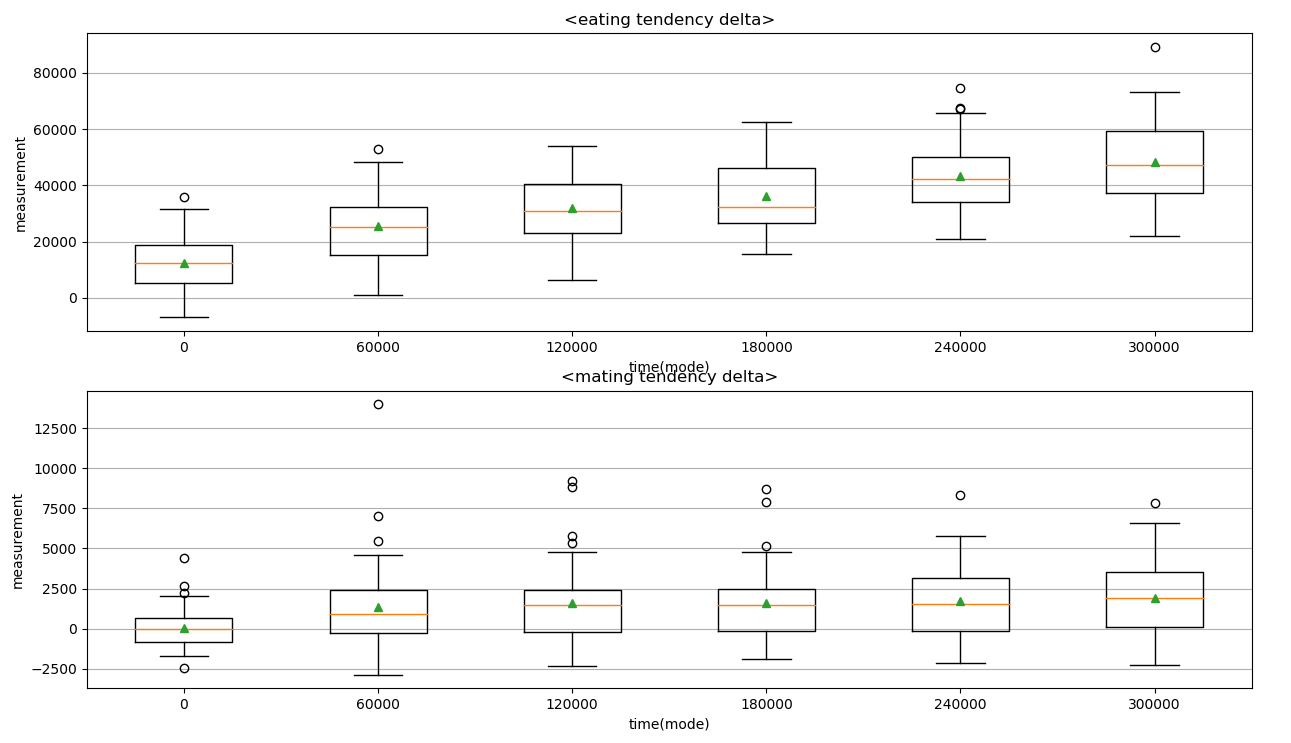
\includegraphics[scale=0.3]{images/main2.png}
\end{center}
\begin{table}[htb]
\begin{tabular}{lllllll}
time & 0 & 60000 & 120000 & 180000&240000&300000 \\
$n$&60&51&50&50&50&49 \\
$p$-value&1.28e-14&4.02e-20&1.35e-23&9.34e-25&5.6e-29&8.21e-28\\
$n$&60&51&50&50&50&49  \\
$p$-value&0.68&7.17e-04&5.26e-05&1.48e-05&1.77e-06&1.17e-07  
  
\end{tabular}
\end{table}

\begin{table}[htb]
\begin{tabular}{lllllll}
time & 0 & 60000 & 120000 & 180000&240000&300000 \\
effect size& 12267& 25565& 32019& 36238& 43264& 48266 \\
average size& 320022&386453&411488&428514&451590&470202\\
ratio& \bf{0.038}& \bf{0.066}& \bf{0.078}& \bf{0.085}& \bf{0.096}& \bf{0.103}\\
effect size& 66& 1342& 1569& 1578& 1712& 1894  \\
average size& 29963& 28589& 28521& 27802& 27097& 26426\\
ratio& \bf{0.002}& \bf{0.047}& \bf{0.055}& \bf{0.057}& \bf{0.063}& \bf{0.072}  
  
\end{tabular}
\end{table}
In the first diagram, the blue boxplots represent the performance distribution of the normal creatures, who are made out of a gene pool obtaind from a simulation at the corresponding time period, while the red ones represent that  of input-shuffled creatures, who are made out of the same gene pool. The second diagram shows the distribution of the performance difference. The p-values in the first table is obtained from the data for the second diagram, using the t-test for mean-zero null hypothesis. The "effect size" in the last table is obtained by averaging the data for the second diagram, and the "average size" is obtaind by averaging the data(blue and red together) for the first daigram. 
  
The result shows that the tendency is statistically significant enough,
and the normalized effect sizes are about 10\% and 7\% respectively for the tasks. 
As we argued before, this shows that the creatures could obtain some proper input-dependent behavioral patterns from the natural evolution of the neural networks. 


\section{discussion}
\subsection{validity of our result}
Some choices as to things such as which features to turn off were made quite arbirarily in the design of experiments. There may still remain some factors that we could not control. Also, as we pointed out earlier, the validity of the mixing input trick depends on the degree to which the input-output functions affects the input distribution. 
\subsection{an episode during the implementation}
When we first developed our simulation program, we observed a consistent bizarre tendency, that the color of the creatures slowly became darker as generation passed, and finally became almost invisible above the black background. At that time, we suspected it as an evicence of intelligence, that forced the creatures to evolve so that the predators cannot detect them. About a month later, after we performed the same simulation with the mixing input trick, we finally realized that it was just an implementation error. In fact, the color of offsprings were biased toward the negative side due to the thoughtless application of python "int" function; it made the color slowly darker stochastically generation after generation. There are two morals of this story. First, a cause identification in this kind of systems is always fragile; a phenomenon may be due to a relatively minor error in the design or implementation detail. Second, to filter out one such alleged cause, it can be useful to devise a controlling method such as our mixing input trick.   
\subsection{future directions}
\subsubsection{Using better neural network models}
In fact, the neural network model used so far is the simplest possible one. There are numerous ways for improvements - adding layers, using convolutional layers and using recursive neural networks. Doing so would increase the effect sizes in the experiments.

\subsubsection{Using more complex virtual ecosystem}
Actually, the virtual ecosystem used in this study was born out of simplifying a much complicated one. The morphology was more complex, which even enabled the creatures to live inside another. The creatures emitted pheromone. The inputs included not only the visual one but also olfactory and somatosensory ones. There were more elaborate "physics" that enabled things such as a crash. It would be very interesting to see whether where the evolution of neural networks leads us to in that ecosystem. 

\subsubsection{checking for predictions of theories of evolution}
Since all basic components of evolution and many features of a living being are already there, we can expect that some directions of evolution that theories of evolution predict under certain environmental circumstances would be also observed in our system.    

\section{appendix A : ecosystem detail}
\subsection{components}
When you run the program, all you see is an empty black space filled with square-shaped  colorful creatures and white nutrients. The creatures can move only parallel to the axes, and the land is assumed to be of toric shape, namely, the left is connected to the right and the bottom is connected to the top. The creatures are born as a result of their parent's mating, interact with each other  and with the environment through 'behaviors', and eventually die to become a collection of nutrients.
\subsection{behaviors}
For how the behavior is determined, see the subsection about neural networks. 
\subsubsection{movement}
It occurs with the amount determined as described in the subsection about neural networks. The movement occurs without any obstruction; the creatures may overlap with each other. 
\subsubsection{eating}
The creature takes up all the nutrients in the pixels it is occupying. When it is of its full size, the size of which is encoded as genotype, the same amount is excreted right away. When it is not of its full size, only a portion of the amount is excreted and the remaining is used for size-up. The rate of excretion is encoded as genotype. The amount of excretion determines the energy taken up, as described later. 
\subsubsection{mating}
When a creature tries mating, its pennis, which occupies only one pixel, appears toward the "moving direction". A trial of mating is done for each other creatures that are occupying the same pixel. Similarity of genes determine the success of mating. If it succeeds, a child is born with the gene determined as described in the subsection about genetics, with the same mass deducted from the mother.
\subsubsection{hunting}
When a creature X tries hunting, all the creatures every occupying pixel of which is also occupied by X suddenly boil down to nutrients, and taken up by X as usual.
\subsection{death}
A creature may die for three different reasons. 
If it dies for one of the first two reasons, a group of nutriets replaces the pixels that the creature has occupied. 
\subsubsection{reaching the life expectancy}
Each creature has its own life expectancy, encoded as genotype.
\subsubsection{using up energy}
Each creature attains energy when they eat, amount proportional to the amount of excretion. Each of the behaviors require certain amounts of energy. In addition to it, there is basal metabolism that consumes a certain amount of energy for each time interval. 
\subsubsection{being hunted}
This is obvious. 

\subsection{genetics}
Creatures have 4 different types of genotypes: life expectancy, subsume-excretion rate during the growing-up period, maximum size and weights of neural networks. All genotypes except for the last consists of one positive real number, while the last is encoded as an array of real numbers. When two genes produce that of the offspring, two stages are involved.
\subsubsection{random mixture}
The first three types of genotypes are just chosen randomly from either of the parents. The weights of the neural networks, on the other hand, are segmented according to the output variable they are connected to, and the random mixture happens in the level of segments. 
\subsubsection{mutation}
Mutation occurs for each real number comprising the gene, with the degree sampled from the Gaussian distribution of mean zero and a fixed standard deviation. 


\section{appendix B : neural network detail}
\subsection{input}
The range of vision is the square whose side length is five times that of the creature and which is centered in the center of the creature's body. Input colors are taken from a square grid equidistanted within the range of vision with a fixed number of vertices.(Therefore, the distance between the neighboring vertices vary with the size of the creature) All r,g,b values are used.   
\subsection{output}
The output consist of 12 quantities. First 4 determine the direction of movement when it occurs. The probability of each direction is calculated using a softmax function. Next 4 numbers determine the distance of movement. Each number, after passed to a sigmoid function, represents the distance when a movement occurs toward the corresponding direction. The last 4 determine one of the behaviors - "move", "eat", "try intercourse" and "try hunt".  
\subsection{network} 
It is simply a linear function, weights initialized uniformly in the interval (-1,1) for the initial creatures.


\section{appendix C : other measurements}
\subsection{population trend}
\begin{center}
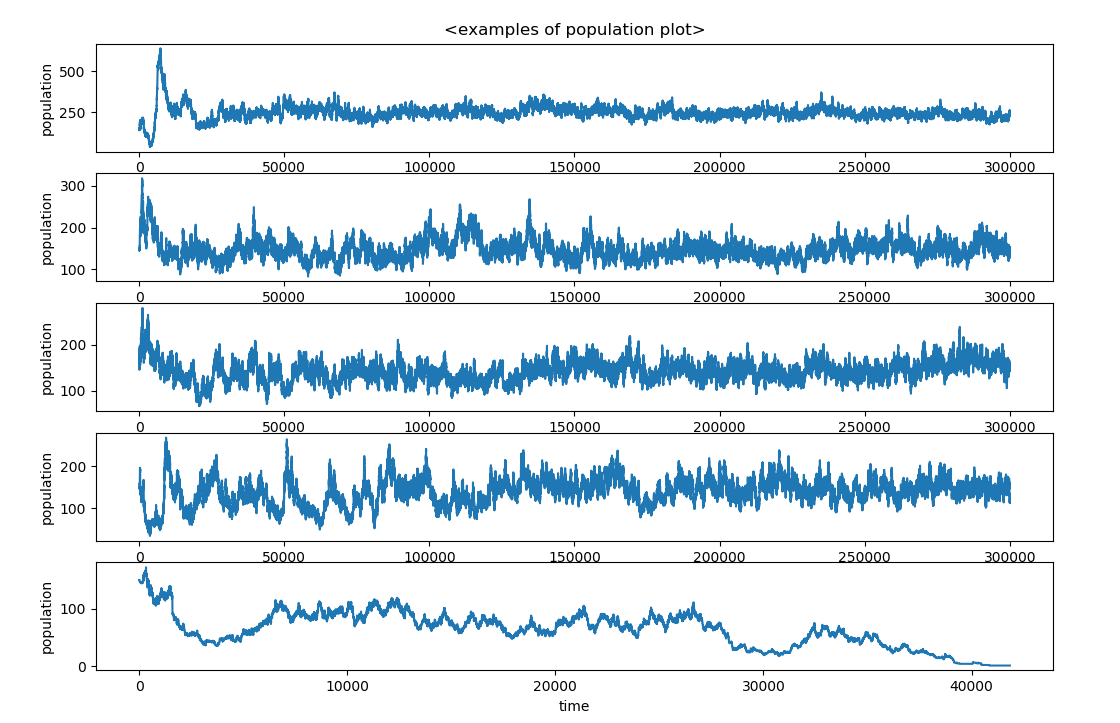
\includegraphics[scale=0.3]{images/population.png}
\end{center}
These are plots of the population in sample runs. 

\subsection{other traits}
\begin{center}
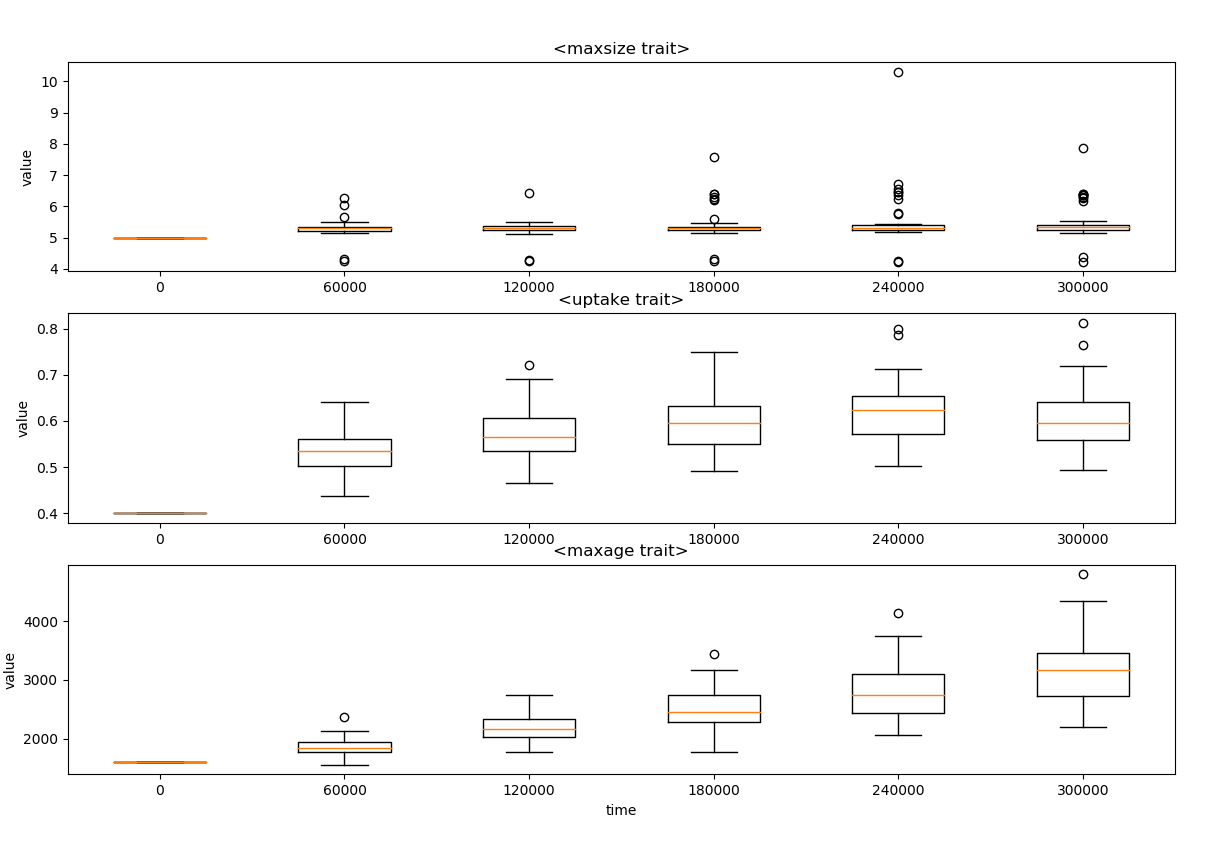
\includegraphics[scale=0.3]{images/traits.png}
\end{center}
These are plots for the distributions of traits other than the weights of neural networks, obtained from the same simulation trials used in the main experiments. 


\subsection{selective pressure}
In a run of 300000s long, numbers of descendents of creatures born before 200000 are counted. 
\begin{table}[htb]
\begin{tabular}{lllll}
number of descendants&0&1$\sim$371&372$\sim$134135&134136$\sim$\\
frequency&154464&92508&0&47877
\end{tabular}
\end{table}

Only about 16\% of the population turned out to have permanent influence on the gene pool, which shows there is a substantial amount of selective pressure. The population that have bounded number of descendents and that have permanent effect on the gene pool are analyzed in more detail in the following figures. The first figure show that among the permanent influencers, the influence slmost precisely depend on the time they were born, which shows their genes quickly became a part of the entire population. The second one shows that most of those failed to become a permanent influencer could not go through the 40 descendants barrier.
\begin{center}
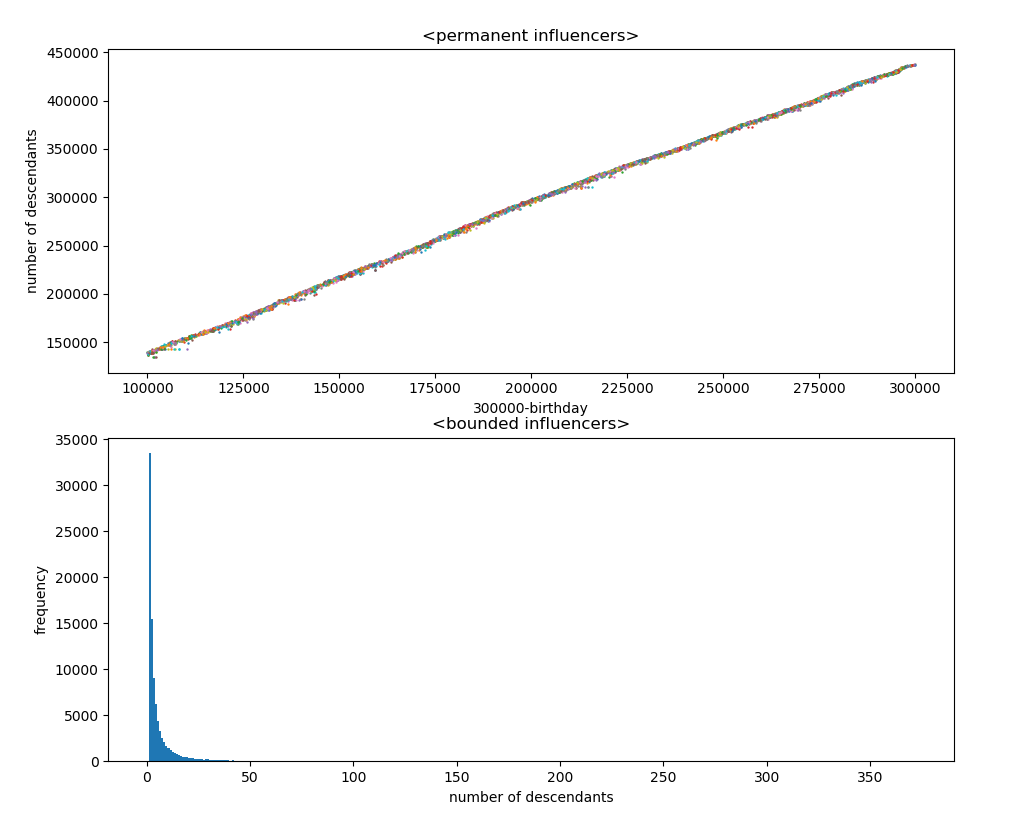
\includegraphics[scale=0.3]{images/detail.png}
\end{center}



%------------------------------------
\bibliographystyle{alpha}
\bibliography{bib.bib}
%------------------------------------------------------
\end{document}


